\documentclass[12pt,oneside,a4paper,reqno]{report}
\usepackage[english]{babel}
\usepackage[utf8x]{vietnam}
% package for including graphics with figure-environment
\usepackage{graphicx}
\usepackage{amsmath,amssymb,exscale,eucal,amsthm, mathrsfs}

%\DeclareMathSizes{12}{15}{9}{9}
\usepackage[table,xcdraw]{xcolor}
\usepackage{tabularx}
\usepackage{longtable}

\usepackage[portrait, top=3.5 cm, bottom=3cm, left=3.5cm, right=2cm] {geometry}
% colors for hyperlinks
% colored borders (false) colored text (true)
\usepackage{wrapfig}
\usepackage{color}
%\usepackage{caption}
% package for bibliography
%\usepackage[round, sort, numbers]{natbib}
% package for header
 

\setlength{\baselineskip}{16truept}
%\renewcommand{\baselinestretch}{1.45}
%%
\renewcommand{\baselinestretch}{1.5}%%đổi về 1.5
%\renewcommand{\baselineskip{1.5}}


\usepackage{enumitem}
%===========thư viện cho header và footer==================
\usepackage{fancyhdr}
\pagestyle{fancy}
%====================================================
\rhead{\textbf{\emph{Đào Tuấn Anh, Vũ Thanh Tùng - KSTN TOÁN TIN K57}}}
\lhead{}
\lfoot{\textbf{Tìm hiểu về SNMP và công cụ giám sát mạng}}
\cfoot{}
\rfoot{\thepage}
\renewcommand{\headrulewidth}{0.4pt}
\renewcommand{\footrulewidth}{0.4pt}
%=====================================================


\begin{document}
\begin{large}

	\begin{titlepage}
\begin{longtable}{p{4cm}p{2cm}p{7cm}}
\centerline{\bf TRƯỜNG ĐẠI HỌC BÁCH KHOA HÀ NỘI}\\
\centerline{\bf VIỆN TOÁN ỨNG DỤNG VÀ TIN HỌC}\\
\centerline{\bf -----------------*-----------------}\\
\end{longtable}

\vspace*{1 cm}

\begin{center}

\includegraphics[width=0.1\textwidth]{images/bkhn.jpg}
\end{center}

\vspace*{1cm}
\centerline{\large\bf BÁO CÁO BÀI TẬP LỚN}

\centerline{\large\bf Môn: Thiết kế, cài đặt và quản trị mạng máy tính}
	
\vspace{1cm}
\centerline{\Large\bf  Đề tài: Tìm hiểu về SNMP và công cụ giám sát mạng Cacti}


\vspace*{1cm}

\begin{center}

$
\begin{array}{llll}
\text{Giảng viên hướng dẫn }&\text{:}
&\text{ThS.  Nguyễn Tuấn Dũng}
\\
\text{Sinh viên thực hiện }&\text{:}
&\text{Đào Tuấn Anh (MSSV: 20121178)}
\\
&\text{:}
&\text{Vũ Thanh Tùng (MSSV: 20124917)}
\\
\text{Lớp }&\text{:}&\text{KSTN TOÁN TIN K57}

\end{array}
$

\end{center}

\vfill
\centerline{\large\bf Hà Nội -- Năm 2016}
\vspace*{0.3cm}
\end{titlepage}
	
\newpage
\tableofcontents
\newpage
	

%%
\newpage
\vspace*{0.2cm}
\centerline{\Large\bf LỜI MỞ ĐẦU}
\vspace*{0.5cm}
\addcontentsline{toc}{chapter}{\bf LỜI MỞ ĐẦU}

Sự phát triển không ngừng nghỉ của công nghệ thông tin đã tạo ra những thay đổi lớn trong cơ sở hạ tầng, lực lượng sản xuất, tính chất lao động, cấu trúc kinh tế và cả cách thức quản lý trong các lĩnh vực của xã hội. Một trong những yếu tố quyết định trong đó, cũng là một nhu cầu tất yếu là việc trao đổi thông tin giữa các thiết bị thông qua mạng máy tính. Sự tăng nhanh về kích cỡ của các hệ thống mạng đã và đang đưa ra thách thức không nhỏ cho người quản trị trong việc theo dõi và quản lý.

Do đó, các hệ thống giám sát an toàn mạng ra đời, đóng vai trò quan trọng, không thể thiếu trong hạ tầng công nghệ thông tin của các cơ quan, đơn vị, tổ chức. Hệ thống này cho phép thu thập, chuẩn hóa, lưu trữ và phân tích tương quan toàn bộ các sự kiện được sinh ra trong hệ thống mạng của tổ chức. Từ đó người quản trị có thể dễ dàng đưa ra phân tích, thống kê, cảnh báo, nắm bắt thực trạng tài nguyên, khắc phục sự cố, đồng thời ngăn chặn sớm các mối nguy hiểm cho hệ thống.

Nội dung dưới đây có đề cập đến giao thức quản lý mạng SNMP (Simple Network Management Protocol). SNMP là một tập hợp các giao thức không chỉ cho phép kiểm tra các thiết bị mạng như router, switch hay server có đang vận hành mà còn hỗ trợ vận hành các thiết bị này một cách tối ưu, ngoài ra SNMP còn cho phép quản lý các thiết bị mạng từ xa. Bên cạnh đó, báo cáo còn đề cập đến Cacti, một hệ thống quản lý tài nguyên mạng mã nguồn mở. Phần mềm này đáp ứng nhu cầu quản lý mạng một cách toàn diện với nhiều tính năng linh hoạt vượt trội.

Em xin chân thành cảm ơn thầy Nguyễn Tuấn Dũng đã tận tình truyền đạt kiến thức trong suốt môn học. Tuy nhiên trong khoảng thời gian cho phép, việc nghiên cứu và trình bày không thể tránh khỏi nhầm lẫn thiếu sót, em mong nhận được sự giúp đỡ đóng góp của thầy cô và bạn bè để bài báo cáo được hoàn thiện hơn.



%---------------------------------------------------
%---------------------------------------------------
\chapter{Tìm hiểu về giao thức SNMP}
\section{Tổng quan về quản lý hệ thống mạng}
\subsection{Khái niệm quản lý hệ thống mạng}
Quản lý hệ thống mạng là việc thực hiện tập hợp các chức năng cần thiết cho việc kiểm soát, lập kế hoạch, phân bổ, triển khai, phối hợp và giám sát các nguồn tài nguyên trong hệ thống. Nó thường được áp dụng cho các mạng quy mô lớn như mạng máy tính và mạng viễn thông, đề cập đến việc duy trì và quản trị mạng ở cấp cao nhất.
\subsection{Khái niệm giám sát mạng}
Giám sát mạng là việc sử dụng một hệ thống liên tục theo dõi hoạt động của một mạng máy tính, thông báo ngay lập tức và cho phép người quản trị mạng biết trong trường hợp xảy ra sự cố ảnh hưởng đến tốc độ hoặc lỗi mạng.

Giám sát mạng là một phần trong quản lý hệ thống mạng.

Một hệ thống giám sát mạng sẽ theo dõi hệ thống mạng gây ra bởi quá tải hay máy chủ bị sập, bởi các kết nối trong mạng hoặc từ các thiết bị khác. Các thông số đánh giá thường gặp là thời gian phản hồi, hiệu lực và thời gian vận hành tối thiểu trung bình (uptime). Ngoài ra còn có các thông số phổ biến khác như độ ổn định hay độ tin cậy.

Ví dụ, để kiểm tra một máy chủ Web, phần mềm giám sát sẽ gửi đều đặn các truy vấn HTTP để lấy nội dung trang web. Ở các máy chủ thư, các gói tin kiểm tra sẽ được gửi đều đặn thông qua SMTP, và nhận lại qua IMAP hoặc POP3.
\subsection{Hai phương thức giám sát mạng: Poll và Alert}
Hai giao thức giám sát “Poll” và “Alert” là 2 phương thức cơ bản của các kỹ thuật giám sát hệ thống, nhiều phần mềm và giao thức được xây dựng dựa trên 2 phương thức này, trong đó có SNMP.

\textbf{Phương thức Poll}

\begin{center}
	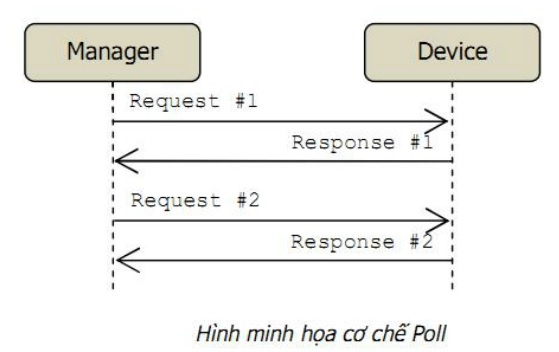
\includegraphics[scale=0.5]{images/poll.jpg}
\end{center}

Nguyên tắc hoạt động: Trung tâm giám sát (manager) sẽ thường xuyên hỏi thông tin của các thiết bị cần giám sát (device). Nếu manager không hỏi thì device không trả lời, nếu manager hỏi thì device trả lời. Bằng cách hỏi thường xuyên, manager sẽ luôn cập nhật được thông tin mới nhất từ device.

\textbf{Phương thức Alert}
\begin{center}
	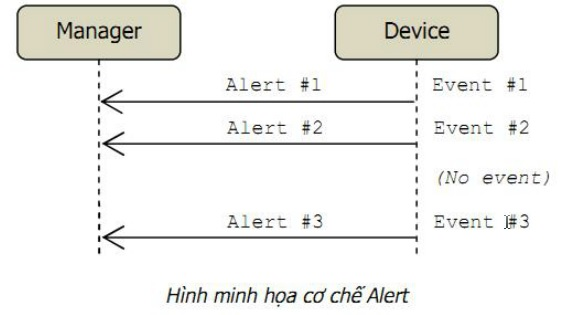
\includegraphics[scale=0.5]{images/alert.jpg}
\end{center}
Nguyên tắc hoạt động: Mỗi khi trong device xảy ra một sự kiện (event) nào đó thì device sẽ tự động gửi thông báo cho Manager, gọi là alert. Manager không hỏi thông tin định kỳ từ device.

Device chỉ gửi những thông báo mang tính sự kiện chứ không gửi những thông tin thường xuyên thay đổi, nó cũng sẽ không gửi Alert nếu chẳng có sự kiện gì xảy ra. Chẳng hạn khi một port down/up thì Device sẽ gửi cảnh báo, còn tổng số byte truyền qua port đó sẽ không được Device gửi đi vì đó là thông tin thường xuyên thay đổi. Muốn lấy những thông tin thường xuyên thay đổi thì Manager phải chủ động đi hỏi device, tức là phải thực hiện phương thức Poll.

\textbf{So sánh 2 phương thức Poll và Alert}

Hai phương thức Poll và Alert là hoàn toàn khác nhau về cơ chế. Một ứng dụng giám sát có thể sử dụng Poll hoặc Alert, hoặc cả hai, tùy vào yêu cầu cụ thể trong thực tế.

Bảng sau so sánh những điểm khác biệt của 2 phương thức:

\begin{longtable}{|p{8cm}|p{8cm}|}
\hline
\rowcolor[HTML]{EFEFEF} 
\multicolumn{1}{|c|}{\cellcolor[HTML]{EFEFEF}\textbf{POLL}}                                                                                                                                                                                                    & \multicolumn{1}{c|}{\cellcolor[HTML]{EFEFEF}\textbf{ALERT}}                                                                                                                                                                                   \\ \hline
Có thể chủ động lấy những thông tin cần thiết từ các đối tượng mình quan tâm, không cần lấy những thông tin không cần thiết từ những nguồn không quan tâm.                                                                                                     & Tất cả những event xảy ra đều được gửi về Manager. Manager phải có cơ chế lọc những event cần thiết, hoặc Device phải thiết lập được cơ chế chỉ gửi những event cần thiết.                                                                    \\ \hline
Có thể lập bảng trạng thái tất cả các thông tin của Device sau khi poll qua một lượt các thông tin đó.                                                                                                                                                         & Nếu không có event gì xảy ra thì Manager không biết được trạng thái của Device.                                                                                                                                                               \\ \hline
Trong trường hợp đường truyền giữa Manager và Device xảy ra gián đoạn và Device có sự thay đổi, thì Manager sẽ không thể cập nhật. Tuy nhiên khi đường truyền thông suốt trở lại thì Manager sẽ cập nhật được thông tin mới nhất do nó luôn luôn poll định kỳ. & Khi đường truyền gián đoạn và Device có sự thay đổi thì nó vẫn gửi Alert cho Manager, nhưng Alert này sẽ không thể đến được Manager. Sau đó mặc dù đường truyền có thông suốt trở lại thì Manager vẫn không thể biết được những gì đã xảy ra. \\ \hline
Chỉ cần cài đặt tại Manager để trỏ đến tất cả các Device. Có thể dễ dàng thay đổi một Manager khác.                                                                                                                                                            & Phải cài đặt từng Device để trỏ đến Manager. Khi thay đổi Manager thì phải cài đặt lại trên tất cả Device để trỏ về Manager mới.                                                                                                              \\ \hline
Nếu tần suất poll thấp, thời gian chờ giữa 2 chu kỳ poll dài sẽ làm Manager chậm cập nhật các thay đổi của Device. Nghĩa là nếu thông tin Device đã thay đổi nhưng vẫn chưa đến lượt poll kế tiếp thì Manager vẫn giữ thông tin cũ.                            & Ngay khi có sự kiện xảy ra thì Device sẽ gửi Alert đến Manager, do đó Manager luôn luôn có thông tin mới nhất tức thời.                                                                                                                       \\ \hline
Có thể bỏ sót các sự kiện : khi Device có thay đổi, sau đó thay đổi trở lại như ban đâu trước khi đến lượt poll kế tiếp thì Manager sẽ không phát hiện được.                                                                                                   & Manager sẽ được thông báo mỗi khi có sự kiện xảy ra ở Device, do đó Manager không bỏ sót bất kỳ sự kiện nào.                                                                                                                                  \\ \hline
\end{longtable}

\section{Giao thức quản lý mạng SNMP (Simple Network Management Protocol)}
\subsection{Giới thiệu giao thức SNMP}
SNMP (viết tắt từ tiếng Anh: Simple Network Management Protocol) là {\it giao thức quản lý mạng đơn giản}.

Rõ thêm, giao thức là một tập hợp các thủ tục mà các bên tham gia cần tuân theo để có thể giao tiếp được với nhau. Trong lĩnh vực thông tin, một giao thức quy định cấu trúc, định dạng của dòng dữ liệu trao đổi với nhau và quy định trình tự, thủ tục để trao đổi dòng dữ liệu đó. Nếu một bên tham gia gửi dữ liệu không đúng định dạng hoặc không theo trình tự thì các bên khác sẽ không hiểu hoặc từ chối trao đổi thông tin. SNMP là một giao thức, do đó nó có những quy định riêng mà các thành phần trong mạng phải tuân theo. Một thiết bị hiểu được và hoạt động tuân theo giao thức SNMP được gọi là “có hỗ trợ SNMP” (SNMP supported) hoặc “tương thích SNMP” (SNMP compartible).

SNMP dùng để quản lý mạng, nghĩa là nó được thiết kế để chạy trên nền TCP/IP và quản lý các thiết bị có kết nối mạng TCP/IP. Các thiết bị mạng không nhất thiết phải là máy tính mà có thể là switch, router, firewall, ADSL gateway, và cả một số phần mềm cho phép quản trị bằng SNMP.

Giao thức SNMP sẽ giải quyết được các bài toán về giám sát tài nguyên máy chủ; giám sát hiệu năng, lưu lượng trên các thiết bị mạng; hệ thống cảnh báo sự cố tức thời.

SNMP là giao thức đơn giản, do nó được thiết kế đơn giản trong cấu trúc bản tin và thủ tục hoạt động, bảo mật. Sử dụng phần mềm SNMP, người quản trị mạng có thể quản lý, giám sát tập trung từ xa toàn mạng của mình.
\subsection{Ưu nhược điểm của giao thức SNMP}

\textbf{Ưu điểm của thiết kế SNMP}

+)SNMP được thiết kế đơn giản hóa quá trình quản lý các thành phần trong mạng. Nhờ đó các phần mềm SNMP có thể được phát triển nhanh và tốn ít chi phí.

+)SNMP được thiết kế có thể mở rộng các chức năng quản lý, giám sát. Không có giới hạn rằng SNMP có thể quản lý được cái gì. Khi có một thiết bị mới với các thuộc tính, tính năng mới thì người ta có thể thiết kế “custom” SNMP để phục vụ cho riêng mình.

+)SNMP được thiết kế có thể hoạt động độc lập với các kiến trúc và cơ chế của các thiết bị hỗ trợ SNMP. Các thiết bị khác nhau có hoạt động khác nhau nhưng đáp ứng SNMP là giống nhau.

\textbf{Nhược điểm của SNMP}

+)Làm tăng lưu lượng đáng kể.

+)Không có sự điều khiển tổng hợp của nhiều nơi quản lý.
\subsection{Các phiên bản giao thức SNMP}
SNMP có 4 phiên bản: SNMPvl, SNMPv2c, SNMPv2u và SNMPv3. Các phiên bản này khác nhau một chút ớ định dạng bán tin và phương thức hoạt động. Hiện tại SNMPvl là phổ biến nhất do có nhiều thiết bị tương thích nhất và có nhiều phần mềm hồ trợ nhất. Trong khi đó chỉ có một số thiết bị và phần mềm hỗ trợ SNMPv3. 
\subsection{Các thành phần chính của giao thức SNMP}
Theo RFC1157, kiến trúc của SNMP bao gồm 2 thành phần: các trạm quản lý mạng (Network Management Station) và các thành tố mạng (Network Element) 3. Network Management Station thường là một máy tính chạy phần mềm quản lý SNMP (SNMP management application), dùng để giám sát và điều khiển tập trung các network element.
\subsection{Kiến trúc giao thức SNMP}
\subsection{Các cơ chế bảo mật trong SNMP}


\chapter{Công cụ giám sát mạng Cacti}
\section{Giới thiệu về công cụ giám sát mạng Cacti}
\section{Kiến trúc phần mềm Cacti}
\section{Cài đặt Cacti trên Windows}
\section{Triển khai và ứng dụng Cacti trong giám sát mạng}
\subsection{Mô hình triển khai}
\subsection{Cấu hình Cacti}

\newpage
\vspace*{0.2cm}
\centerline{\Large\bf KẾT LUẬN CHUNG}
\vspace*{0.5cm}
\addcontentsline{toc}{chapter}{\bf KẾT LUẬN CHUNG}

\newpage
\vspace*{0.2cm}
\centerline{\Large\bf TÀI LIỆU THAM KHẢO}
\vspace*{0.5cm}
\addcontentsline{toc}{chapter}{\bf TÀI LIỆU THAM KHẢO}

%\bibliographystyle{ksfh_nat}
%	\bibliography{references} % expects file "references.bib"
\begin{enumerate}
\item{Wikipedia, "Simple Network Management Protocol", https://en.wikipedia.org/wiki/SNMP}
\item{Wikipedia, "Network monitoring", https://en.wikipedia.org/wiki/Network\_monitoring}
\item{TBT - VNCERT, "Tổng quan về hệ thống giám sát mạng", http://www.vncert.gov.vn/}
\item{Diệp Thanh Nguyên, "SNMP Toàn tập", https://sites.google.com/site/snmptoantap/home}
\end{enumerate}
	
\end{large}		

\end{document}